\chapter{Discussion}\label{chap:discussion}


\subsection{\textbf{Creating the LSTM models}}

    The following report includes all the steps that we followed in order to create a working LSTM model. The dataset will be archived and sent with this report. Prerequisites are a code editor (Spyder, VSCode), stable version of Python "2.7 >" and git on a local machine.
    First, we need to clone the repository. Link to the repository is:
    \href{https://github.com/LauraWartschinski/VulnerabilityDetection}{Repo}. After executing "git clone" command, we can get a glimpse of the projects file structure. It is recommended to use python's virtual environment for installing all necessary packages for safety reasons.
    Setting up virtual environment in Python3 is easy and straightforward process and it works by executing this command "python3 -m venv myenv". Now we need to activate the venv we created in the previous step with this command "source path/to/env". 
    
    \begin{figure}
        \centering
        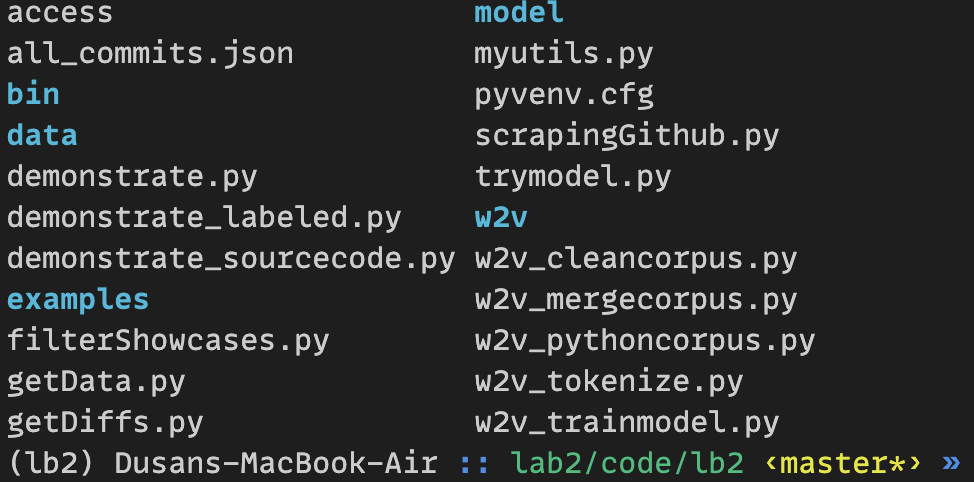
\includegraphics[width=0.5\linewidth]{Screenshot 2024-05-12 at 09.38.43.png}
        \caption{File structure}
        \label{fig:enter-label}
    \end{figure}

\newpage

    After we verified that our development environment is functional, we can proceed to the next steps.
    \begin{itemize}
     \item 1 Usage of scrapingGithub.py
     \item 2 Usage of filterShowcases.py
      \item 3 Usage of getDiffs.py
      \item 4 Usage of getData.py sql
       \item 5 Usage of makemodel.py sql
    \end{itemize}
    
    \textbf{scrapingGithub.py} script is used for gathering and downloading different commits. For this script to work, we need to provide an access token. Access token can be found on github setting page. Now
    it is necessary to create a file called "access" in the same directory and paste the provided key. On line 10 of "scrapingGithub.py" script
    there is a function searchForKeyword(). SearchForKeyword() function  
    takes 3 parameters "key" , "commit" , "success". Variable "maximum", on the line of code 12, represents number of repositories that will be scraped and the default value is "9999". After executing the script,
    shortly afterwards, we are prompted with a response that indicated a successful scraping procedure. All results are saved in allcommits.json() file that we are required to create prior to executing the script. If the file is not created accordingly, the following error message is printed in the terminal "The file is empty or does not exist".
    
     \begin{figure}
        \centering
        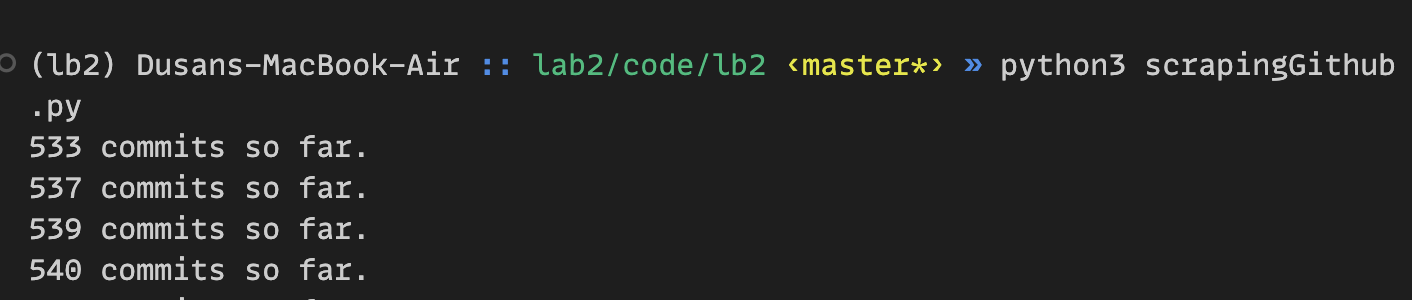
\includegraphics[width=0.5\linewidth]{Screenshot 2024-05-12 at 10.42.04.png}
        \caption{Gathering repositories}
        \label{fig:enter-label}
    \end{figure}
\newpage

    \textbf{filterShowcase.py} script is used for filtering all repositories that are not suitable for the dataset. Certain repositories are used for "Capture the Flag" challenges or vulnerability demonstration which are already vulnerable by default.
    Variable repositories on the line of code 7 is initialized as an empty collection of objects. Diving further into the code, we can confirm that data loads from open() function (line of code 13) that opens a file and returns a text stream. Previously created text stream is then saved into DataFilter.json file. Array of strings with specific keywords can be further altered to match our search criteria. Example can be found on lines of code 29 and 30.
     \begin{itemize}
     \item toomuchsecurity = ['offensive', 'pentest', 'vulnerab', 'security', 'hack', 'exploit', 'ctf ', ' ctf', 'capture the flag','attack'] 
     \item alittletoomuch = ['offensive security', 'pentest', 'exploits', 'vulnerability research', 'hacking', 'security framework', 'vulnerability database', 'simulated attack', 'security research'] 
     \end{itemize}
    Now we can demonstrate the functionality of this script by running the following command "python3 filterShowcase.py". If compilation error persists on first execution, its mandatory to install python library "OS" with the command "pip3 install os"
    
    \begin{figure}
            \centering
            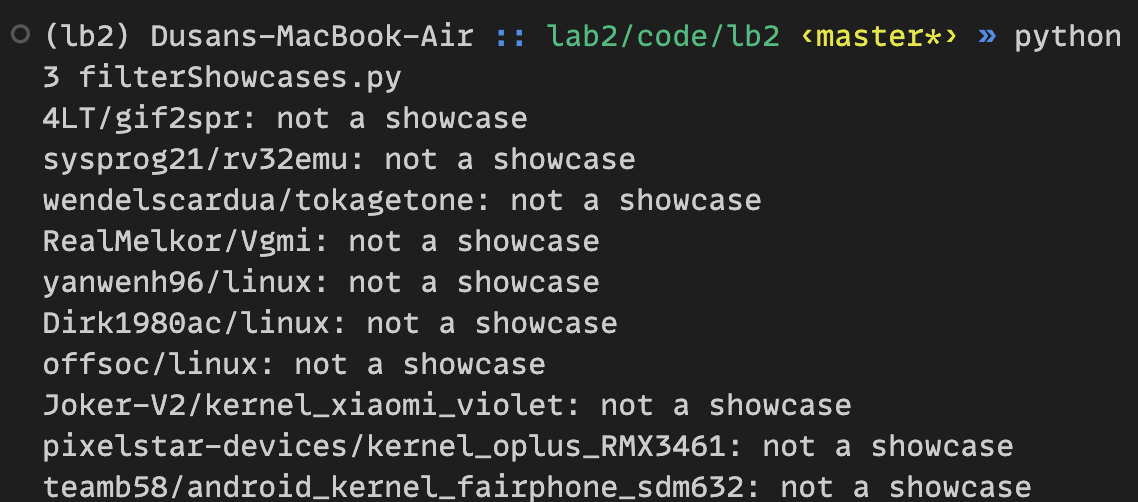
\includegraphics[width=1\linewidth]{Screenshot 2024-05-12 at 11.48.39.png}
            \caption{Filtering repositories}
            \label{fig:enter-label}
        \end{figure}

    \textbf{getDiffs.py} script is used to further modify already filtered data. Executing this script returns the data that is further processed into PyCommitsWithDiffs.json file. The script analyzes the code and finds whether the repositories contain python code or not. Repositories without python code are labeled as "don't contain python", and repositories that contain python are labeled as "contain python". Showcases are ignored and filtered out. In our demonstration there are 500+ repositories previously gathered. Now, we can get required data for creating our models from PyCommitsWithDiffs.json file. PyDriller library is a vital part of getData.py script which creates the crucial data for model training step. Functionality of getData.py script will be explained in the next steps.
    
    \begin{figure}
        \centering
        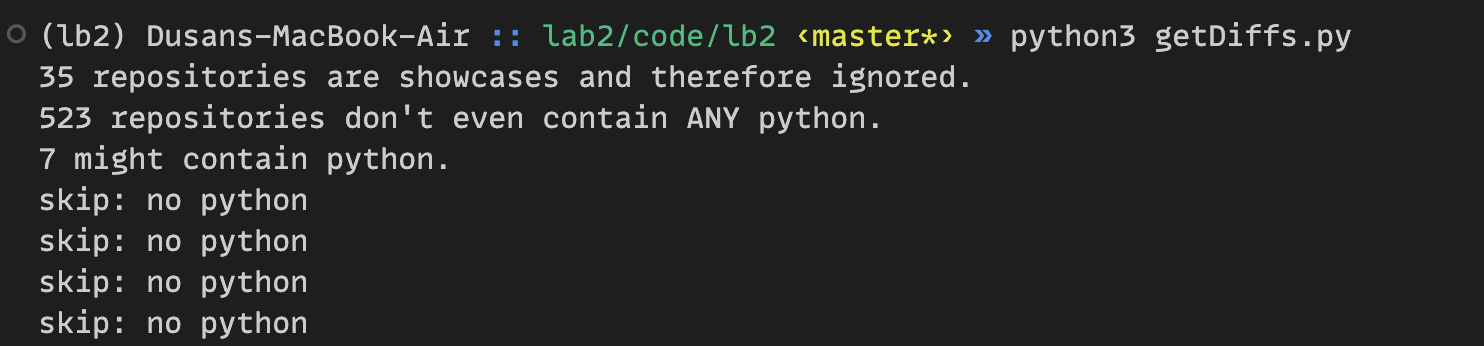
\includegraphics[width=1\linewidth]{Screenshot 2024-05-12 at 12.04.05.png}
        \caption{Further filtering with getDiffs.py}
        \label{fig:enter-label}
    \end{figure}

    \textbf{getData.py}
    *We must remember that there are some changes in the PyDriller library since it was used for this repository. The changes are as follows:
\begin{enumerate}
    \item The \textit{RepositoryMinning} class changed to \textit{Repository} \newline \textbf{Repository} is the main class of Pydriller, responsible for returning the list of commits you want. One of the main advantages of using PyDriller to mine software repositories is that it is highly configurable. We will now see all the options one can pass to the Repository.
\newpage
\end{enumerate}


    \textbf{getData.py} script reads all the repositories from PyCommitsWithDiffs.json file and downloads all crucial source code required for the next steps. Also, it prepares all parameters for making the models and executes getChanges(),getFileName(),makechangeobj(), functions. 
    For this script to efficiently work, we had to execute all the previous steps and wait for the scripts to finish. On the line of code 9, PyDriller import is changed to "from pydriller import Repository". Now we can utilize Repository class to return the list of all commits. Executing this script involves time dependency of n(repositories) mined from the previous steps. Result is saved to "data" folder.
    On the line of code 317, RepositoryMining class is changed to Repository(r).
    
    \begin{figure}
            \centering
            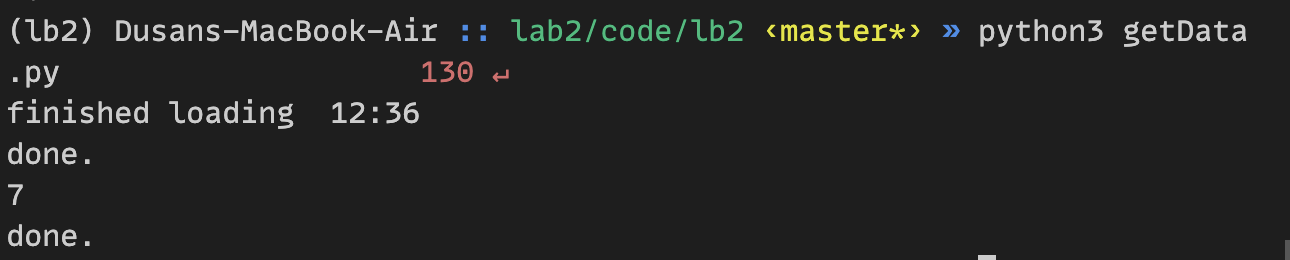
\includegraphics[width=1\linewidth]{Screenshot 2024-05-12 at 12.39.27.png}
            \caption{getData.py}
            \label{fig:enter-label}
        \end{figure}
                

   \textbf{makemodel.py} script is used for creating data models. It splits the data in 3 different segments (train, validate, final).
   On the line of code 134, the samples are randomized with \textbf{for} loop. However, there are certain issues regarding this code. Library \textbf{Keras} that is imported in myutils.py file is causing a build error. Keras package is now \textbf{included} in previous installation of tensorflow package. Therefore, imports needed to be adjusted accordingly. "from keras.datasets import imdb" is now "tensorflow.keras.datasets". Also, we need to install all necessary packages (gensim, sklearn, tensorflow). Next, datasets are created using word2vec models created in previous exercise. Unfortunately, new error occurs where we need to adjust 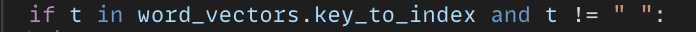
\includegraphics[width=0.5\linewidth]{Screenshot 2024-05-12 at 13.10.36.png} this line of code to match the new key to index parameter. Console is clear from errors so we can proceed to make our new vulnerability model. After loading the data, script creates new training dataset 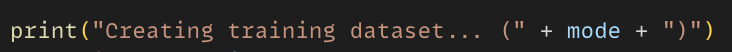
\includegraphics[width=0.5\linewidth]{Screenshot 2024-05-12 at 13.14.57.png}, followed by 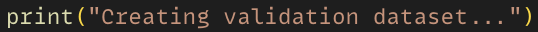
\includegraphics[width=0.5\linewidth]{Screenshot 2024-05-12 at 13.16.00.png} and finally 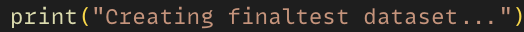
\includegraphics[width=0.5\linewidth]{Screenshot 2024-05-12 at 13.16.43.png}.
                  
   %   \begin{figure}
   %     \centering
   %     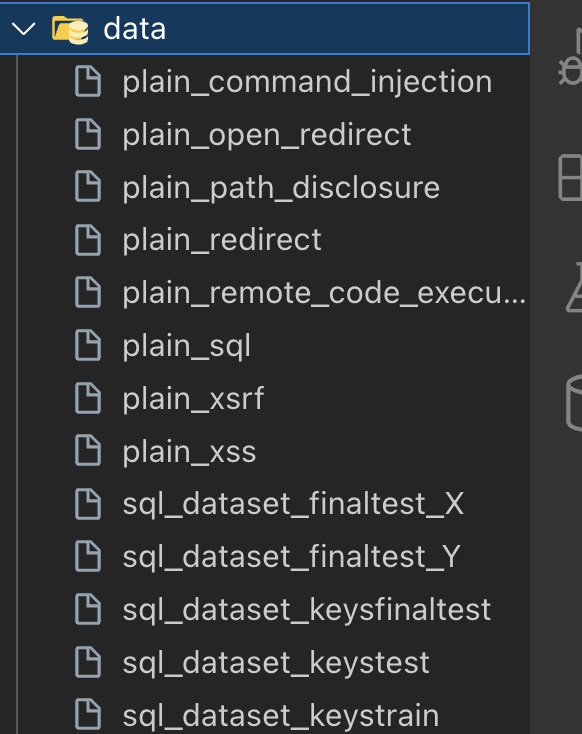
\includegraphics[width=0.5\linewidth]{Screenshot 2024-05-12 at 12.41.42.png}
   %     \caption{Folder structure with data}
   %     \label{fig:enter-label}
   % \end{figure}                               


  % add the console output of final steps
  % adjust the images
  % format the document 
   
   